\documentclass[xcolor=table]{beamer}
\usepackage{amsmath,amsthm}
\usepackage{amssymb}
\usepackage[english]{babel}
\usepackage{latexsym}
\usepackage{amsfonts}
\usepackage{graphicx}
\usepackage{float}
\usepackage{tikz}
\usepackage{graphics}
\usetikzlibrary{arrows.meta,arrows,shapes,positioning,shadows,trees,calc}

\usepackage{epsfig}
\usepackage{hyperref}
\usepackage{url}
\usepackage{multirow}
\usetheme{Madrid} 
\useoutertheme{miniframes}
% Custom commands for consistency
\newcommand\independent{\protect\mathpalette{\protect\independenT}{\perp}}
\def\independenT#1#2{\mathrel{\rlap{$#1#2$}\mkern2mu{#1#2}}}

% https://arxiv.org/pdf/1907.07271
% https://economics.mit.edu/sites/default/files/inline-files/causal_tutorial_1.pdf
% https://ocw.mit.edu/courses/14-03-microeconomic-theory-and-public-policy-fall-2016/1a8bade59dad1809321428afef18074e_MIT14_03F16_lec2.pdf


% Consistent TikZ style
\tikzset{
    causal/.style={-{Latex[length=4mm, width=2mm]}, thick, blue},
    node/.style={draw, circle, minimum size=0.8cm},
    highlight/.style={fill=yellow!20},
    blocked/.style={->, >=stealth, thick, red, dashed}
}

\mode<presentation>

\title{Causal Concepts Illustrated with DAGs}
\author{Diomides Mavroyiannis}
\date{\today}

\begin{document}

\begin{frame}
    \titlepage
\end{frame}

\begin{frame}{Outline}
    \tableofcontents
\end{frame}


\begin{frame}{Roadmap: Building Causal Understanding}
    \begin{center}
        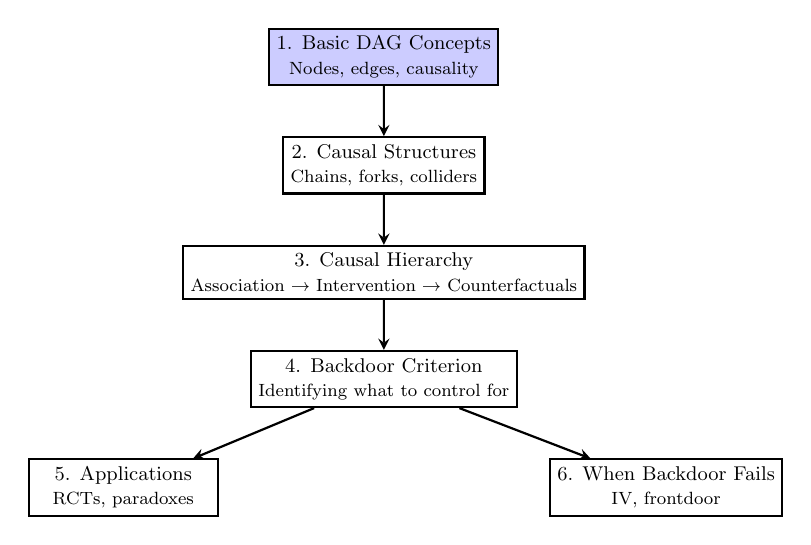
\begin{tikzpicture}[
            scale=0.80, transform shape,
            node distance=0.8cm,
            box/.style={rectangle, draw, thick, minimum width=3cm, minimum height=0.8cm, align=center, font=\small},
            arrow/.style={->, thick, >=stealth},
            highlight/.style={fill=blue!20}
        ]
            % Level 1
            \node[box, highlight] (basics) {1. Basic DAG Concepts\\{\footnotesize Nodes, edges, causality}};
            
            % Level 2
            \node[box, below=of basics] (structures) {2. Causal Structures\\{\footnotesize Chains, forks, colliders}};
            
            % Level 3
            \node[box, below=of structures] (hierarchy) {3. Causal Hierarchy\\{\footnotesize Association → Intervention → Counterfactuals}};
            
            % Level 4
            \node[box, below=of hierarchy] (backdoor) {4. Backdoor Criterion\\{\footnotesize Identifying what to control for}};
            
            % Level 5 - split
            \node[box, below left=0.8cm and 0.5cm of backdoor] (applications) {5. Applications\\{\footnotesize RCTs, paradoxes}};
            \node[box, below right=0.8cm and 0.5cm of backdoor] (alternatives) {6. When Backdoor Fails\\{\footnotesize IV, frontdoor}};
            
            % Arrows
            \draw[arrow] (basics) -- (structures);
            \draw[arrow] (structures) -- (hierarchy);
            \draw[arrow] (hierarchy) -- (backdoor);
            \draw[arrow] (backdoor) -- (applications);
            \draw[arrow] (backdoor) -- (alternatives);
            
            
        \end{tikzpicture}
    \end{center}
\end{frame}

\section{Introduction to Causality}

\begin{frame}{Causality and Empiricism}
    \begin{itemize}
        \item Directed Acyclic Graphs (DAGs) represent causal relationships
        \item The general term for these relationships is \textbf{association}
        \item \textbf{Correlation} is a special kind of association
    \end{itemize}
    
    \vspace{0.5cm}
    
    \begin{block}{Key Insight}
        The following two causal structures are empirically identical - no associative measure can distinguish between them:
    \end{block}
    
    \begin{center}
        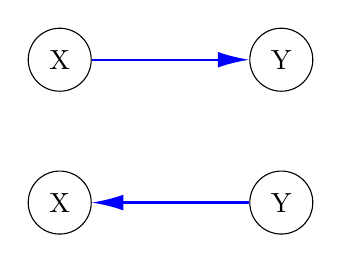
\begin{tikzpicture}[node distance=2cm]
            % First structure: X -> Y
            \node[node] (x1) {X};
            \node[node, right=of x1] (y1) {Y};
            \draw[causal] (x1) -- (y1);
            
            % Second structure: Y -> X
            \node[node, below=1cm of x1] (x2) {X};
            \node[node, right=of x2] (y2) {Y};
            \draw[causal] (y2) -- (x2);
        \end{tikzpicture}
    \end{center}
\end{frame}

\section{Basic DAG Concepts}

\begin{frame}{Introduction to DAGs}
    \begin{itemize}
        \item \textbf{Directed Acyclic Graphs (DAGs)} represent causal relationships
        \item \textbf{Nodes} = variables
        \item \textbf{Edges} = causal relationships (direction matters)
        \item \textbf{No cycles} allowed (cannot be both cause and effect of itself)
    \end{itemize}
    
    \vspace{0.5cm}
    
    \begin{center}
        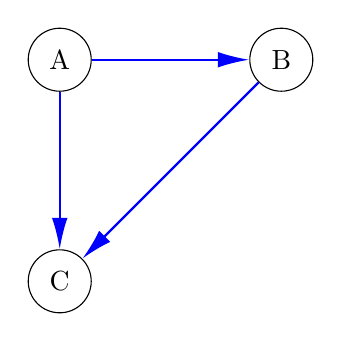
\begin{tikzpicture}[node distance=2cm]
            \node[node] (A) {A};
            \node[node, right=of A] (B) {B};
            \node[node, below=of A] (C) {C};
            \draw[causal] (A) -- (B);
            \draw[causal] (A) -- (C);
            \draw[causal] (B) -- (C);
        \end{tikzpicture}
    \end{center}
    
    \begin{block}{Reading the Graph}
        X causes both C and Y directly, while B also causes Y
    \end{block}
\end{frame}

\begin{frame}{Example: Free Will vs Determinism: Four Philosophical Positions}
    \begin{center}
        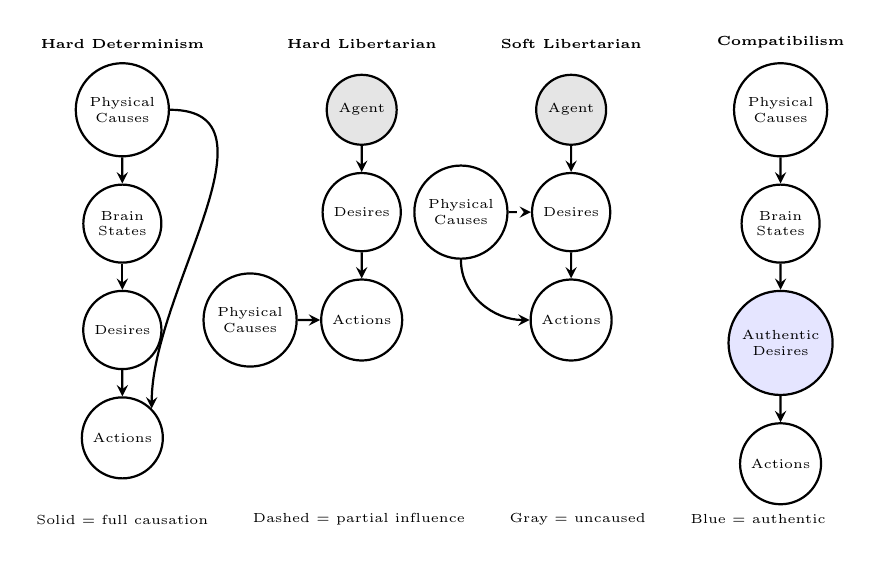
\begin{tikzpicture}[
            scale=0.95, transform shape,
            node distance=0.35cm,
            node/.style={circle, draw, thick, minimum size=0.6cm, align=center, font=\tiny},
            causal/.style={->, thick, >=stealth},
            weak/.style={->, thick, >=stealth, dashed},
            title/.style={font=\tiny\bfseries, above=0.3cm}
        ]
            
            % Hard Determinism
            \node[title] at (0, 0) {Hard Determinism};
            \node[node] (p1) at (0, -0.4) {\tiny Physical\\Causes};
            \node[node, below=of p1] (b1) {\tiny Brain\\States};
            \node[node, below=of b1] (d1) {\tiny Desires};
            \node[node, below=of d1] (a1) {\tiny Actions};
            
            \draw[causal] (p1) -- (b1);
            \draw[causal] (b1) -- (d1);
            \draw[causal] (d1) -- (a1);
            \draw[causal] (p1.east) to[out=0, in=90] (a1.north east);
            
            % Hard Libertarian Free Will
            \node[title] at (3.2, 0) {Hard Libertarian};
            \node[node, fill=gray!20] (ag2) at (3.2, -0.4) {\tiny Agent};
            \node[node, below=of ag2] (d2) {\tiny Desires};
            \node[node, below=of d2] (a2) {\tiny Actions};
            \node[node, left=0.3cm of a2] (p2) {\tiny Physical\\Causes};
            
            \draw[causal] (ag2) -- (d2);
            \draw[causal] (d2) -- (a2);
            \draw[causal] (p2) -- (a2);
            
            % Soft Libertarian Free Will
            \node[title] at (6, 0) {Soft Libertarian};
            \node[node, fill=gray!20] (ag3) at (6, -0.4) {\tiny Agent};
            \node[node, below=of ag3] (d3) {\tiny Desires};
            \node[node, below=of d3] (a3) {\tiny Actions};
            \node[node, left=0.3cm of d3] (p3) {\tiny Physical\\Causes};
            
            \draw[causal] (ag3) -- (d3);
            \draw[weak] (p3) -- (d3);
            \draw[causal] (d3) -- (a3);
            \draw[causal] (p3) to[out=-90, in=180] (a3.west);
            
            % Compatibilism
            \node[title] at (8.8, 0) {Compatibilism};
            \node[node] (p4) at (8.8, -0.4) {\tiny Physical\\Causes};
            \node[node, below=of p4] (b4) {\tiny Brain\\States};
            \node[node, below=of b4, fill=blue!10] (d4) {\tiny Authentic\\Desires};
            \node[node, below=of d4] (a4) {\tiny Actions};
            
            \draw[causal] (p4) -- (b4);
            \draw[causal] (b4) -- (d4);
            \draw[causal] (d4) -- (a4);
            
            % Legend at bottom
            \node[font=\tiny, below= of a1](l1) {Solid = full causation};
            \node[font=\tiny, right= of l1](l2) {Dashed = partial influence};
            \node[font=\tiny, right= of l2](l3) {Gray = uncaused};
            \node[font=\tiny, right= of l3](l4){Blue = authentic};
            
        \end{tikzpicture}
    \end{center}
\end{frame}

\begin{frame}{Necessary Causes}
    \begin{columns}
        \begin{column}{0.6\textwidth}
            \begin{itemize}
                \item A cause is \textbf{necessary} for an effect if the effect cannot occur without the cause
                \item Logical Form: $\neg X \rightarrow \neg Y$
                \item Entailment 1: $P(X) \geq P(Y)$ 
                \item Entailment 2: $P(Y|\neg X) =0$
            \end{itemize}
            
            \vspace{0.5cm}
            
            \begin{exampleblock}{Example}
                Oxygen is necessary for fire - without oxygen, combustion cannot occur
            \end{exampleblock}
        \end{column}
        \begin{column}{0.4\textwidth}
            \begin{center}
                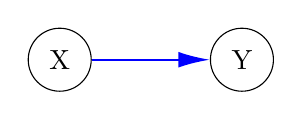
\begin{tikzpicture}[node distance=1.5cm]
                    \node[node] (X) {X};
                    \node[node, right=of X] (Y) {Y};
                    \draw[causal] (X) -- (Y);
                \end{tikzpicture}
            \end{center}
        \end{column}
    \end{columns}
\end{frame}

\begin{frame}{Sufficient Causes}
    \begin{columns}
        \begin{column}{0.6\textwidth}
            \begin{itemize}
                \item A cause is \textbf{sufficient} for an effect if the cause guarantees the effect
                \item Logical Form: $ X \rightarrow Y$
                \item Entailment 1: $P(X) \leq P(Y)$
                \item Entailment 2: $P(Y|X) = 1$
            \end{itemize}
            
            \vspace{0.5cm}
            
            \begin{exampleblock}{Example}
                Being a triangle is sufficient for being a polygon - every triangle is necessarily a polygon
            \end{exampleblock}
        \end{column}
        \begin{column}{0.4\textwidth}
            \begin{center}
                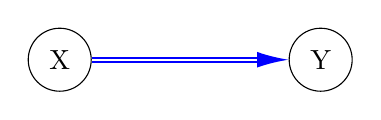
\begin{tikzpicture}[node distance=2.5cm]
                    \node[node] (X) {X};
                    \node[node, right=of X] (Y) {Y};
                    \draw[causal, double] (X) -- (Y);
                \end{tikzpicture}
            \end{center}
            \small{Double arrow indicates sufficiency}
        \end{column}
    \end{columns}
\end{frame}

\begin{frame}{Overdetermination}
    \begin{columns}
        \begin{column}{0.6\textwidth}
            \begin{itemize}
                \item \textbf{Overdetermination} occurs when multiple causes independently can bring about the effect
                \item Form: $(X \rightarrow Y) \land (C \rightarrow Y)$ 
                \item Entailment: $P(Y) \geq max(P(X), P(C))$
            \end{itemize}
            
            \vspace{0.5cm}
            
            \begin{exampleblock}{Example}
                Multiple gunshots - any single shot would be sufficient to cause death
            \end{exampleblock}
        \end{column}
        \begin{column}{0.4\textwidth}
            \begin{center}
                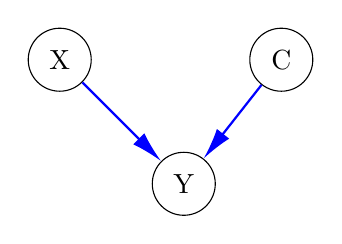
\begin{tikzpicture}[node distance=2cm]
                    \node[node] (X) {X};
                    \node[node, right=2cm of X] (C) {C};
                    \node[node, below right=1cm and 1cm of X] (Y) {Y};
                    \draw[causal] (X) -- (Y);
                    \draw[causal] (C) -- (Y);
                \end{tikzpicture}
            \end{center}
        \end{column}
    \end{columns}
\end{frame}

\begin{frame}{Underdetermination}
    \begin{columns}
        \begin{column}{0.6\textwidth}
            \begin{itemize}
                \item \textbf{Underdetermination} occurs when multiple causes are jointly necessary but individually insufficient for the effect.
                \item Form: $(X \land C) \rightarrow Y$, but $\neg(X \rightarrow Y)$ and $\neg(C \rightarrow Y)$.
                \item Entailment: \\ $P(Y|X \land C) \gg P(Y|X), P(Y|C)$, \\ with $P(Y|X) \approx 0$ and $P(Y|C) \approx 0$.
            \end{itemize}

            
            \vspace{0.5cm}
            
            \begin{exampleblock}{Example}
                Fire requires both oxygen and fuel - neither alone is sufficient to produce fire
            \end{exampleblock}
        \end{column}
        \begin{column}{0.4\textwidth}
            \begin{center}
                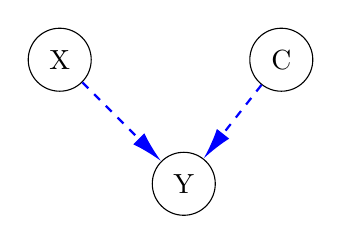
\begin{tikzpicture}[node distance=2cm]
                    \node[node] (X) {X};
                    \node[node, right=2cm of X] (C) {C};
                    \node[node, below right=1cm and 1cm of X] (Y) {Y};
                    \draw[causal, dashed] (X) -- (Y);
                    \draw[causal, dashed] (C) -- (Y);
                \end{tikzpicture}
            \end{center}
        \end{column}
    \end{columns}
\end{frame}

\section{Causal Structures}


\begin{frame}{The Four Basic Causal Structures}
    \begin{align*}
        (X \not\independent Y) \parallel Z \text{ or } (X \independent Y) \parallel Z
    \end{align*}
    
    \vspace{0.3cm}
    
    \begin{center}
        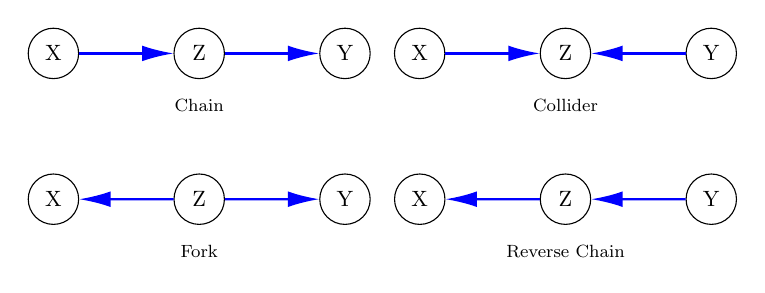
\begin{tikzpicture}[node distance=1.5cm, scale=0.8, transform shape]
            % Chain: X -> Z -> Y
            \node[node] (x1) {X};
            \node[node, right=of x1] (z1) {Z};
            \node[node, right=of z1] (y1) {Y};
            \draw[causal] (x1) -- (z1);
            \draw[causal] (z1) -- (y1);
            \node[below=0.2cm of z1] {\footnotesize Chain};
            
            % Fork: Z -> X, Z -> Y
            \node[node, below=1.5cm of z1] (z2) {Z};
            \node[node, left=of z2] (x2) {X};
            \node[node, right=of z2] (y2) {Y};
            \draw[causal] (z2) -- (x2);
            \draw[causal] (z2) -- (y2);
            \node[below=0.2cm of z2] {\footnotesize Fork};
            
            % Collider: X -> Z <- Y
            \node[node, right=5cm of x1] (x3) {X};
            \node[node, right=of x3] (z3) {Z};
            \node[node, right=of z3] (y3) {Y};
            \draw[causal] (x3) -- (z3);
            \draw[causal] (y3) -- (z3);
            \node[below=0.2cm of z3] {\footnotesize Collider};
            
            % Mixed: Z -> X, Y -> Z
            \node[node, below=1.5cm of z3] (z4) {Z};
            \node[node, left=of z4] (x4) {X};
            \node[node, right=of z4] (y4) {Y};
            \draw[causal] (z4) -- (x4);
            \draw[causal] (y4) -- (z4);
            \node[below=0.2cm of z4] {\footnotesize Reverse Chain};
        \end{tikzpicture}
    \end{center}
\end{frame}



\begin{frame}{Causal Chains (Mediation)}
    \begin{columns}
        \begin{column}{0.6\textwidth}
            \begin{itemize}
                \item \textbf{Causal Chains} show mediated relationships
                \item X causes Z which causes Y
                \item X is an \textbf{indirect cause} of Y
                \item Z \textbf{mediates} the relationship between X and Y
            \end{itemize}
            
            \vspace{0.5cm}
            
            \begin{exampleblock}{Example}
                Education → Skills → Income\\
                Education affects income through developing skills
            \end{exampleblock}
        \end{column}
        \begin{column}{0.4\textwidth}
            \begin{center}
                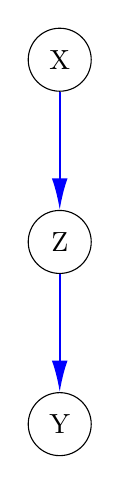
\begin{tikzpicture}[node distance=1.5cm]
                    \node[node] (X) {X};
                    \node[node, below=of X] (Z) {Z};
                    \node[node, below=of Z] (Y) {Y};
                    \draw[causal] (X) -- (Z);
                    \draw[causal] (Z) -- (Y);
                \end{tikzpicture}
            \end{center}
        \end{column}
    \end{columns}
\end{frame}

\begin{frame}{Common Cause (Confounding)}
    \begin{columns}
        \begin{column}{0.6\textwidth}
            \begin{itemize}
                \item A \textbf{Common Cause} can create a spurious correlation
                \item Z causes both X and Y
                \item X and Y appear correlated but have no direct causal relationship
            \end{itemize}
            
            \vspace{0.5cm}
            
            \begin{exampleblock}{Example}
                Summer weather causes both ice cream sales and drowning deaths - they're correlated but neither causes the other
            \end{exampleblock}
        \end{column}
        \begin{column}{0.4\textwidth}
            \begin{center}
                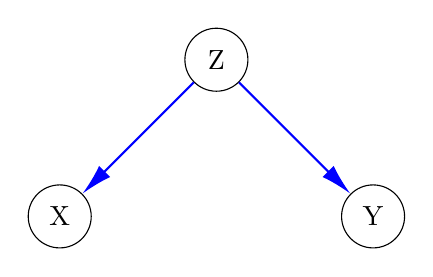
\begin{tikzpicture}[node distance=2cm]
                    \node[node] (Z) {Z};
                    \node[node, below left=of Z] (X) {X};
                    \node[node, below right=of Z] (Y) {Y};
                    \draw[causal] (Z) -- (X);
                    \draw[causal] (Z) -- (Y);
                \end{tikzpicture}
            \end{center}
        \end{column}
    \end{columns}
\end{frame}



\begin{frame}{Colliders}
    \begin{columns}
        \begin{column}{0.6\textwidth}
            \begin{itemize}
                \item A \textbf{Collider} is where multiple causes influence a common effect
                \item Unlike common causes, conditioning on a collider can \textbf{create} spurious correlations
                \item X and Y are independent until we condition on Z
            \end{itemize}
            
            \vspace{0.5cm}
            
            \begin{exampleblock}{Example}
                Intelligence and work ethic both cause success - among successful people, these traits appear negatively correlated
            \end{exampleblock}
        \end{column}
        \begin{column}{0.4\textwidth}
            \begin{center}
                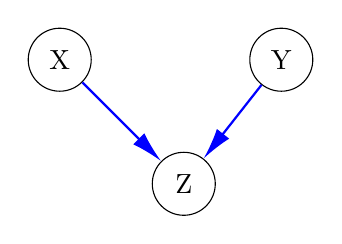
\begin{tikzpicture}[node distance=2cm]
                    \node[node] (X) {X};
                    \node[node, right=2cm of X] (Y) {Y};
                    \node[node, below right=1cm and 1cm of X] (Z) {Z};
                    \draw[causal] (X) -- (Z);
                    \draw[causal] (Y) -- (Z);
                \end{tikzpicture}
            \end{center}
        \end{column}
    \end{columns}
\end{frame}



\section{The Causal Hierarchy}


\begin{frame}{The Causal Hierarchy: Three Levels of Reasoning}
    \begin{block}{Pearl's Causal Hierarchy}
        Three distinct levels of causal reasoning, each more powerful than the last
    \end{block}
    
    \begin{enumerate}
        \item \textbf{Association (Seeing/Observing)}
        \begin{itemize}
            \item What is? How are variables related?
            \item $P(Y|X)$ - conditional probability
            \item Purely statistical, no causal claims
        \end{itemize}
        
        \item \textbf{Intervention (Doing/Acting)}
        \begin{itemize}
            \item What if I do? What happens if we change X?
            \item $P(Y|do(X))$ - interventional probability
            \item Requires causal knowledge beyond correlation
        \end{itemize}
        
        \item \textbf{Counterfactuals (Imagining)}
        \begin{itemize}
            \item What if things had been different?
            \item $P(Y_x|X' \neq x)$ - probability Y would be y if X had been x
            \item Requires most complete causal understanding
        \end{itemize}
    \end{enumerate}
    
\end{frame}

\begin{frame}{Level 1: Association and Observation}
    \textbf{Mathematical Framework}
    \begin{itemize}
        \item Joint distribution: $P(X,Y)$
        \item Conditional probability: $P(Y|X) = \frac{P(X,Y)}{P(X)}$
        \item Independence: $X \independent Y \iff P(Y|X) = P(Y)$
    \end{itemize}
    
    \textbf{What We Can Answer}
    \begin{itemize}
        \item "What is the probability of disease given symptom?"
        \item "Are education and income correlated?"
        \item "What patterns exist in the data?"
    \end{itemize}

    
    \begin{center}
        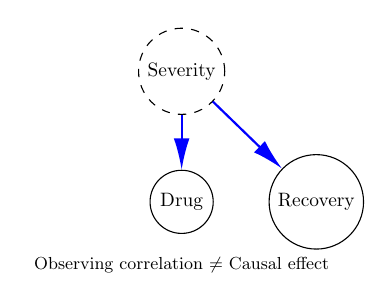
\begin{tikzpicture}[node distance=1cm, scale=0.7, transform shape]
            \node[node] (x) {Drug};
            \node[node, right=of x] (y) {Recovery};
            \node[node, above=of x, dashed] (z) {Severity};
            \draw[causal] (z) -- (x);
            \draw[causal] (z) -- (y);
            \node[below=0.3cm of x] {\small Observing correlation $\neq$ Causal effect};
        \end{tikzpicture}
    \end{center}
\end{frame}

\begin{frame}{Levels 2 Intervention (do-calculus)}
    \textbf{Level 2: }
    \begin{itemize}
        \item $P(Y|do(X=x))$ - probability of Y when we set X to x
        \item Differs from conditioning: $P(Y|do(X=x)) \neq P(Y|X=x)$ in general
        \item Answers: "What if we force everyone to take the drug?"
    \end{itemize}
    
    \begin{columns}
        \begin{column}{0.5\textwidth}
            \centering
            $P(Y|X=x)$\\
            \vspace{0.2cm}
            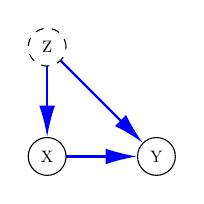
\begin{tikzpicture}[node distance=1.5cm, scale=0.6, transform shape]
                \node[node] (x) {X};
                \node[node, right=of x] (y) {Y};
                \node[node, above=of x, dashed] (z) {Z};
                \draw[causal] (z) -- (x);
                \draw[causal] (z) -- (y);
                \draw[causal] (x) -- (y);
            \end{tikzpicture}
        \end{column}
        \begin{column}{0.5\textwidth}
            \centering
            $P(Y|do(X=x))$\\
            \vspace{0.2cm}
            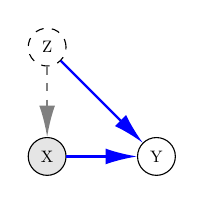
\begin{tikzpicture}[node distance=1.5cm, scale=0.6, transform shape]
                \node[node, fill=gray!20] (x) {X};
                \node[node, right=of x] (y) {Y};
                \node[node, above=of x, dashed] (z) {Z};
                \draw[causal, gray, dashed] (z) -- (x);
                \draw[causal] (z) -- (y);
                \draw[causal] (x) -- (y);
            \end{tikzpicture}
            \small{(Incoming arrows cut)}
        \end{column}
    \end{columns}
\end{frame}

\begin{frame}{Level 3: Counterfactuals}
    \begin{itemize}
        \item $Y_{x}(u)$ - value Y would take for unit u if X were set to x
        \item Individual Treatment Effect: $\text{ITE}(u) = Y_{1}(u) - Y_{0}(u)$
        \item Answers: "What if this specific patient had taken the drug?"
    \end{itemize}
    
    \begin{block}{What Requires Counterfactuals vs Intervention}
        \textbf{Level 2 (Intervention):}
        \begin{itemize}
            \item ATE = $E[Y|do(X=1)] - E[Y|do(X=0)]$
            \item ATT, CATE (population averages)
        \end{itemize}
        
        \textbf{Level 3 (Counterfactual):}
        \begin{itemize}
            \item ITE for specific individual
            \item "Would X have prevented Y?" (necessity)
            \item "Would X have caused Y?" (sufficiency)
        \end{itemize}
    \end{block}
    
\end{frame}

% Add this slide AFTER the Level 3 Counterfactuals slide

\section{Backdoor Criterion}

\begin{frame}{Backdoor Criterion: Causal Effect of X on Y}
    \begin{block}{Water System Analogy}
        Think of it like a water system. There must not be any indirect paths from X to Y:
        \begin{itemize}
            \item Regular variables are \textbf{open gates} - if controlled, they close
            \item Colliders are \textbf{closed gates} - if controlled, they open
        \end{itemize}
    \end{block}
    
    \begin{block}{Three-Step Process}
        \begin{enumerate}
            \item Draw your DAG
            \item List every backdoor path from X to Y
            \item Find a set of controls such that all backdoor paths are closed
        \end{enumerate}
    \end{block}
\end{frame}

\begin{frame}{Backdoor Example 1}
    \begin{center}
        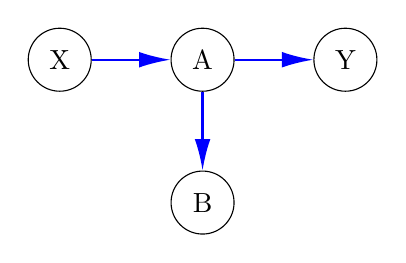
\begin{tikzpicture}[node distance=1cm]
            \node[node] (x) {X};
            \node[node, right=of x] (a) {A};
            \node[node, right=of a] (y) {Y};
            \node[node, below=of a] (b) {B};
            
            \draw[causal] (x) -- (a);
            \draw[causal] (a) -- (y);
            \draw[causal] (a) -- (b);
        \end{tikzpicture}
    \end{center}
    
    \vspace{0.5cm}
    
    \textbf{Control sets:} $\{\emptyset, \{B\}\}$
    
    \begin{block}{Explanation}
        No backdoor paths exist from X to Y, so no controls needed. Controlling for B is also valid but unnecessary.
    \end{block}
\end{frame}

\begin{frame}{Backdoor Example 2}
    \begin{center}
        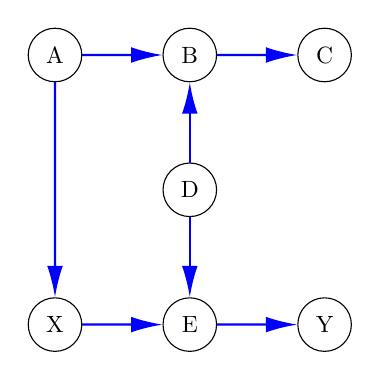
\begin{tikzpicture}[node distance=1.2cm, scale=0.85, transform shape]
            \node[node] (d) {D};
            \node[node, above=of d] (b) {B};
            \node[node, below=of d] (e) {E};
            \node[node, left=of b] (a) {A};
            \node[node, right=of b] (c) {C};
            \node[node, left=of e] (x) {X};
            \node[node, right=of e] (y) {Y};
            
            \draw[causal] (a) -- (x);
            \draw[causal] (a) -- (b);
            \draw[causal] (x) -- (e);
            \draw[causal] (d) -- (b);
            \draw[causal] (d) -- (e);
            \draw[causal] (b) -- (c);
            \draw[causal] (e) -- (y);
        \end{tikzpicture}
    \end{center}
    
    
    \textbf{Control sets:} $\{\emptyset\}$ and all subsets of $\{A,C,D\}$ except $\{B\}$, $\{B,C\}$ and $E$ should never be controlled for. 
    
    
    \begin{block}{Explanation}
        Backdoor path X←A→B←D→E→Y exists, but B is a collider on this path, so it's naturally blocked.
    \end{block}
\end{frame}

\begin{frame}{Backdoor Example 3}
    \begin{center}
        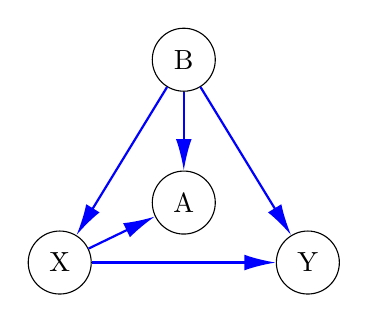
\begin{tikzpicture}[node distance=2cm]
            \node[node] (b) {B};
            \node[node, below left=2cm and 1cm of b] (x) {X};
            \node[node, below right=2cm and 1cm of b] (y) {Y};
            \node[node, below=1 of b] (a) {A};
            
            \draw[causal] (b) -- (x);
            \draw[causal] (b) -- (a);
            \draw[causal] (b) -- (y);
            \draw[causal] (x) -- (a);
            \draw[causal] (x) -- (y);
        \end{tikzpicture}
    \end{center}
    
    \vspace{0.5cm}
    
    \textbf{Control sets:} $\{\{B\}, \{A,B\}\}$
    
    \begin{block}{Explanation}
        Backdoor path X←B→Y must be blocked by controlling for B.
    \end{block}
\end{frame}

\begin{frame}{Backdoor Examples 4 \& 5}
    \begin{center}
        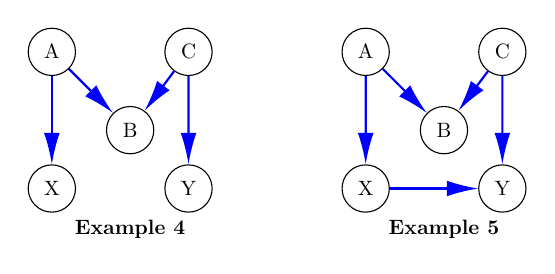
\begin{tikzpicture}[node distance=1.8cm, scale=0.75, transform shape]
            % Example 4
            \node[node] (a1) {A};
            \node[node, below right=0.75cm and 0.75cm of a1] (b1) {B};
            \node[node, right=1.5 of a1] (c1) {C};
            \node[node, below=1.5 of a1] (x1) {X};
            \node[node, below=1.5 of c1] (y1) {Y};
            
            \draw[causal] (a1) -- (x1);
            \draw[causal] (a1) -- (b1);
            \draw[causal] (c1) -- (b1);
            \draw[causal] (c1) -- (y1);
            
            \node[below=1cm of b1] {\textbf{Example 4}};
            
            % Example 5
            \node[node, right=4.5cm of a1] (a2) {A};
            \node[node, below right=0.75 and 0.75 of a2] (b2) {B};
            \node[node, right=1.5 of a2] (c2) {C};
            \node[node, below=1.5 of a2] (x2) {X};
            \node[node, below=1.5 of c2] (y2) {Y};
            
            \draw[causal] (a2) -- (x2);
            \draw[causal] (a2) -- (b2);
            \draw[causal] (c2) -- (b2);
            \draw[causal] (c2) -- (y2);
            \draw[causal] (x2) -- (y2);
            
            \node[below=1cm of b2] {\textbf{Example 5}};
        \end{tikzpicture}
    \end{center}
    
    \vspace{0.3cm}
    
    \begin{itemize}
        \item \textbf{Example 4 and 5 control sets:} $\{\emptyset, \{A,B\}, \{B,C\}, \{A,B,C\}\}$
    \end{itemize}
\end{frame}

\section{Applications and Paradoxes}

\begin{frame}{Simpson's Paradox: Birth Weight Example}
    \begin{block}{Paradox}
        Low birth-weight children born to smoking mothers have a lower infant mortality rate than low birth-weight children of non-smokers.
    \end{block}
    \begin{center}
    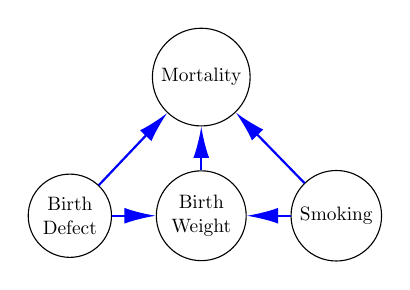
\begin{tikzpicture}[scale=0.70, transform shape, node distance=0.8cm ]
        \node[node, align=center] (weight) {Birth\\Weight};
        \node[node, right=of weight] (smoking) {Smoking};
        \node[node, left=of weight, align=center] (defect) {Birth\\Defect};
        \node[node, above=of weight] (mortality) {Mortality};
        
        \draw[causal] (smoking) -- (weight);
        \draw[causal] (smoking) -- (mortality);
        \draw[causal] (defect) -- (weight);
        \draw[causal] (defect) -- (mortality);
        \draw[causal] (weight) -- (mortality);
    \end{tikzpicture}
    \end{center}
    
    \begin{alertblock}{Explanation}
        Birth weight is a collider - conditioning on it creates spurious correlation between smoking and mortality within the low birth-weight group.
    \end{alertblock}
\end{frame}


\subsection{Experimental Design}
\begin{frame}{Randomized Controlled Trials (RCTs)}
    \begin{columns}
        \begin{column}{0.6\textwidth}
            \begin{itemize}
                \item \textbf{Gold standard} for causal inference
                \item Random assignment breaks all backdoor paths
                \item Creates independence: $Z \independent U$
                \item Eliminates confounding by design
            \end{itemize}
            
            \vspace{0.5cm}
            
            \begin{exampleblock}{Key Properties}
                \begin{itemize}
                    \item Z (assignment) affects X (treatment)
                    \item Z is independent of all confounders U
                    \item Effect identified by comparing groups
                \end{itemize}
            \end{exampleblock}
        \end{column}
        \begin{column}{0.4\textwidth}
            \begin{center}
                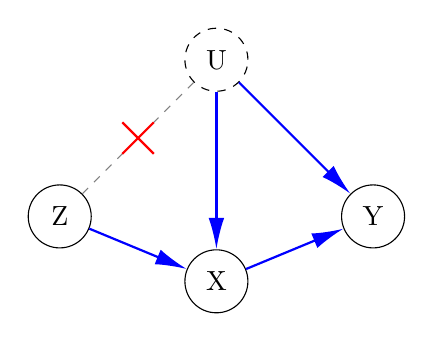
\begin{tikzpicture}[node distance=2cm]
                    \node[node, dashed] (U) {U};
                    \node[node, below left=of U] (Z) {Z};
                    \node[node, below=of U] (X) {X};
                    \node[node, below right=of U] (Y) {Y};
                    
                    \draw[causal] (U) -- (X);
                    \draw[causal] (U) -- (Y);
                    \draw[causal] (Z) -- (X);
                    \draw[causal] (X) -- (Y);
                    
                    % Draw a dashed line between U and Z to show potential path
                    \draw[dashed, gray] (U) -- (Z);
                    
                    % Cross out the dashed path to show it's broken by randomization
                    \coordinate (midpoint) at ($(U)!0.5!(Z)$);
                    \draw[red, thick] ($(midpoint) + (-0.2,-0.2)$) -- ($(midpoint) + (0.2,0.2)$);
                    \draw[red, thick] ($(midpoint) + (-0.2,0.2)$) -- ($(midpoint) + (0.2,-0.2)$);
                \end{tikzpicture}
            \end{center}
            \small{Randomization breaks the U→Z path}
        \end{column}
    \end{columns}
\end{frame}

\begin{frame}{RCTs as Edge-Cutters}
\begin{block}{Key Insight}
Random assignment \textbf{blocks all incoming edges} to the treatment node, except from the randomization device itself.
\end{block}

\begin{itemize}
\item Randomization makes treatment statistically independent of all pre-treatment variables
\item Formally: $P(T | \text{Parents}(T)) \rightarrow P(T | R)$
\item This independence breaks confounding paths
\end{itemize}

\begin{alertblock}{Result}
$T \perp\!\!\!\perp \{U, X, \ldots\} | R$
\end{alertblock}
\end{frame}

%% Slide 2: Visual Representation
\begin{frame}{Visual Representation: Before and After}
\begin{columns}
\column{0.5\textwidth}
\textbf{Observational Setting:}
\begin{center}
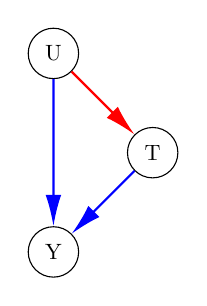
\begin{tikzpicture}[node distance=1.8cm, scale=0.8, transform shape]
\node[node] (U) {U};
\node[node, below right=1cm and 1cm of U] (T) {T};
\node[node, below left=1cm and 1cm of T] (Y) {Y};

\draw[causal, red] (U) -- (T);
\draw[causal] (U) -- (Y);
\draw[causal] (T) -- (Y);
\end{tikzpicture}
\end{center}
\textcolor{red}{Confounding path: $U \rightarrow T \rightarrow Y$}

\column{0.5\textwidth}
\textbf{After Randomization:}
\begin{center}
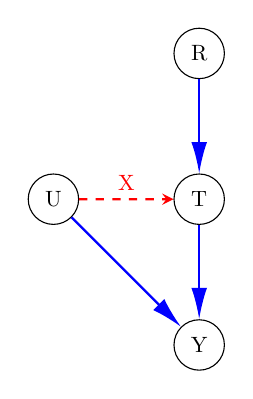
\begin{tikzpicture}[node distance=1.8cm, scale=0.8, transform shape]
\node[node] (R) {R};
\node[node, below=1.5cm of R] (T) {T};
\node[node, left=1.5cm of T] (U) {U};
\node[node, below=1.5cm of T] (Y) {Y};

\draw[causal, blue] (R) -- (T);
\draw[causal] (U) -- (Y);
\draw[causal] (T) -- (Y);
\draw[blocked] (U) -- (T) node[midway, above] {X};
\end{tikzpicture}
\end{center}
\textcolor{blue}{Only path to $T$: through $R$}
\end{columns}
\end{frame}

%% Slide 3: Which Edges Are Affected
\begin{frame}{Which Edges Are Affected?}
\begin{columns}
\column{0.6\textwidth}
\textbf{Edges that ARE blocked:}
\begin{itemize}
\item All edges \textbf{into} treatment from pre-treatment variables
\item Confounding paths through treatment
\item Selection into treatment based on characteristics
\end{itemize}

\vspace{0.5cm}

\textbf{Edges that are NOT blocked:}
\begin{itemize}
\item Edges \textbf{from} treatment to outcomes
\item Direct effects of confounders on outcomes
\item Mediating paths: $T \rightarrow M \rightarrow Y$
\end{itemize}

\column{0.4\textwidth}
\begin{center}
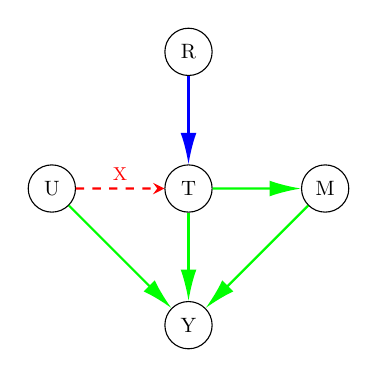
\begin{tikzpicture}[node distance=1.5cm, scale=0.75, transform shape]
\node[node] (R) {R};
\node[node, below=of R] (T) {T};
\node[node, right=of T] (M) {M};
\node[node, below=of T] (Y) {Y};
\node[node, left=of T] (U) {U};

\draw[causal] (R) -- (T);
\draw[causal, green] (T) -- (M);
\draw[causal, green] (M) -- (Y);
\draw[causal, green] (T) -- (Y);
\draw[causal, green] (U) -- (Y);
\draw[blocked] (U) -- (T) node[midway, above] {\small X};
\end{tikzpicture}
\end{center}

\small
\textcolor{red}{Blocked edge} \\
\textcolor{green}{Active edges}
\end{columns}
\end{frame}

%% Slide 4: Mathematical Formulation
\begin{frame}{Mathematical Formulation}
\begin{block}{Independence Achievement}
Randomization achieves: $T \perp\!\!\!\perp \{U, X, \ldots\} | R$
\end{block}

This means:
\begin{align}
\mathbb{E}[Y | T = 1] - \mathbb{E}[Y | T = 0] &= \text{ATE}
\end{align}

\textbf{Why?} No backdoor paths from $T$ to $Y$:
\begin{itemize}
\item All paths $U \rightarrow T \rightarrow Y$ are blocked at the first arrow
\item Only variation in $T$ comes from $R$ (random)
\item Association between $T$ and $Y$ must be causal
\end{itemize}

\begin{alertblock}{Key Assumption}
No interference, perfect compliance, no attrition
\end{alertblock}
\end{frame}

%% Slide 5: Variations in Randomization
\begin{frame}{Variations in Randomization}
\begin{block}{Stratified/Blocked Randomization}
Randomize within levels of $X$: $P(T | X, U) \rightarrow P(T | X, R)$
\end{block}

\begin{center}
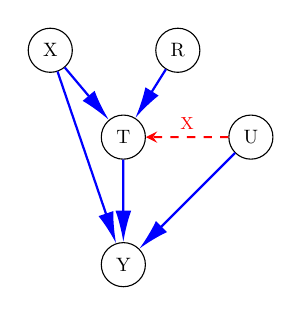
\begin{tikzpicture}[node distance=1cm, scale=0.7, transform shape]
\node[node] (X) {X};
\node[node, right=1.5cm of X] (R) {R};
\node[node, below right=1cm and 0.75cm of X] (T) {T};
\node[node, right=1.5cm of T] (U) {U};
\node[node, below=1.5cm of T] (Y) {Y};

\draw[causal, blue] (X) -- (T);
\draw[causal, blue] (R) -- (T);
\draw[causal] (X) -- (Y);
\draw[causal] (T) -- (Y);
\draw[causal] (U) -- (Y);
\draw[blocked] (U) -- (T) node[midway, above] {\small X};
\end{tikzpicture}
\end{center}

\begin{itemize}
\item Edges from all variables except $X$ and $R$ are cut
\item Must condition on $X$ in analysis
\item Improves precision if $X$ predicts $Y$
\end{itemize}
\end{frame}

%% Slide 6: What RCTs Don't Fix
\begin{frame}{What RCTs Don't Fix}
\begin{alertblock}{Important Limitations}
Randomization only addresses confounding, not other issues:
\end{alertblock}

\begin{enumerate}
\item \textbf{Attrition/Selection Bias:} Post-treatment selection can reopen paths
\item \textbf{Non-compliance:} Creates gap between ITT and ATE
\item \textbf{Measurement Error:} Doesn't fix measurement issues
\item \textbf{External Validity:} Only identifies effects in study population
\end{enumerate}

\vspace{0.5cm}

\begin{block}{Remember}
\begin{itemize}
\item Don't condition on post-treatment variables (reopens paths)
\item Don't control for mediators (blocks part of causal effect)
\item Watch for differential attrition (creates selection bias)
\end{itemize}
\end{block}
\end{frame}

%% Slide 7: Key Takeaways
\begin{frame}{Key Takeaways}
\begin{enumerate}
\item \textbf{RCTs as surgical edge removal:} Randomization precisely cuts confounding edges while preserving causal paths

\vspace{0.3cm}

\item \textbf{Independence is key:} $T \perp\!\!\!\perp \text{Pre-treatment variables} | R$

\vspace{0.3cm}

\item \textbf{Know what's blocked:} 
\begin{itemize}
\item Edges INTO treatment (blocked)
\item Edges FROM treatment (preserved)
\end{itemize}

\vspace{0.3cm}

\item \textbf{Design implications:} Understanding edge-cutting helps design better experiments (stratification, clustering)

\vspace{0.3cm}

\item \textbf{Limitations remain:} RCTs solve confounding but not all causal inference problems
\end{enumerate}
\end{frame}

\begin{frame}{RCTs and Vaccine Drug Trials: Population Mortality Rates}
    \begin{columns}
        \begin{column}{0.6\textwidth}
            \begin{itemize}
                \item \textbf{Critical insight}: Treatment effect depends on baseline mortality rate
                \item Higher severity populations → larger observable effects
                \item Same drug shows different effect sizes across populations
            \end{itemize}
                        
            \begin{alertblock}{Why This Matters}
                Drug preventing 50\% of deaths:
                \begin{itemize}
                    \item If 50\% of population  infected \\ $\rightarrow$ 25\% better than placebo. 
                    \item If 10\% of population  infected \\ $\rightarrow$ 5\% better than placebo.               \end{itemize}
            \end{alertblock}
        \end{column}
        \begin{column}{0.4\textwidth}
            \begin{center}
                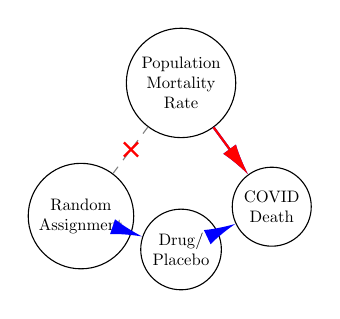
\begin{tikzpicture}[node distance=1.5cm, scale=0.6, transform shape]
                    \node[node, xshift=-4cm, align=center] (pop) {Population\\Mortality\\Rate};
                    \node[node, below left=1.2cm and 0.5cm of pop, align=center] (assign) {Random\\Assignment};
                    \node[node, below=of pop, align=center] (drug) {Drug/\\Placebo};
                    \node[node, below right=1.2cm and 0.5cm of pop, align=center] (outcome) {COVID\\Death};
                    
                    \draw[causal] (pop) -- (outcome);
                    \draw[causal] (assign) -- (drug);
                    \draw[causal] (drug) -- (outcome);
                    
                    % Highlight that population rate affects outcome
                    \draw[causal, red, thick] (pop) -- (outcome);
                    
                    % No connection from population to assignment (key for RCT)
                    \draw[dashed, gray] (pop) -- (assign);
                    \coordinate (midpoint) at ($(pop)!0.5!(assign)$);
                    \draw[red, thick] ($(midpoint) + (-0.15,-0.15)$) -- ($(midpoint) + (0.15,0.15)$);
                    \draw[red, thick] ($(midpoint) + (-0.15,0.15)$) -- ($(midpoint) + (0.15,-0.15)$);
                \end{tikzpicture}
            \end{center}
            \small{Population rate affects outcomes but not assignment}
        \end{column}
    \end{columns}
\end{frame}

\section{Other ways of getting a backdoor}

\begin{frame}{What if you can't close the backdoors?}
    Two options to measure effect of X on Y without closing backdoor:
    
    \vspace{0.3cm}
    
    \begin{columns}
        \begin{column}{0.5\textwidth}
            \begin{center}
                \textbf{Instrumental Variable}
                \vspace{0.2cm}
                
                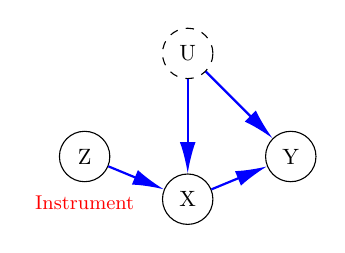
\begin{tikzpicture}[node distance=1.5cm, scale=0.8, transform shape]
                    \node[node, dashed] (u) {U};
                    \node[node, below left=of u] (z) {Z};
                    \node[node, below=of u] (x) {X};
                    \node[node, below right=of u] (y) {Y};
                    
                    \draw[causal] (u) -- (x);
                    \draw[causal] (u) -- (y);
                    \draw[causal] (z) -- (x);
                    \draw[causal] (x) -- (y);
                    
                    % Highlight the instrument
                    \node[below=0.1cm of z, red] {\small Instrument};
                \end{tikzpicture}
                
                \vspace{0.3cm}
                Find something that causes X which doesn't have a backdoor
            \end{center}
        \end{column}
        \begin{column}{0.5\textwidth}
            \begin{center}
                \textbf{Frontdoor Criterion}
                \vspace{0.2cm}
                
                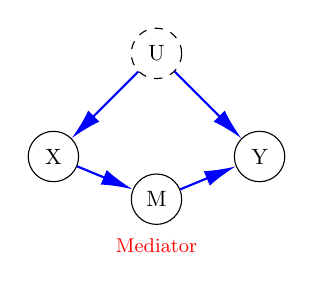
\begin{tikzpicture}[node distance=1.5cm, scale=0.8, transform shape]
                    \node[node, dashed] (u) {U};
                    \node[node, below left=of u] (x) {X};
                    \node[node, below=of u] (m) {M};
                    \node[node, below right=of u] (y) {Y};
                    
                    \draw[causal] (u) -- (x);
                    \draw[causal] (u) -- (y);
                    \draw[causal] (x) -- (m);
                    \draw[causal] (m) -- (y);
                    
                    % Highlight the mediator
                    \node[below=0.1cm of m, red] {\small Mediator};
                \end{tikzpicture}
                
                \vspace{0.3cm}
                Find an intermediary variable between X and Y
            \end{center}
        \end{column}
    \end{columns}
\end{frame}

\begin{frame}{Frontdoor Criterion}
    \begin{columns}
        \begin{column}{0.6\textwidth}
            \begin{itemize}
                \item Used when there are \textbf{unobserved confounders}
                \item M satisfies frontdoor criterion if:
                \begin{enumerate}
                    \item X affects Y only through M (complete mediation)
                    \item No unobserved confounders of X-M relationship
                    \item No unobserved confounders of M-Y relationship (given X)
                \end{enumerate}
            \end{itemize}
            
            
            % \begin{exampleblock}{Key Formula}
            %     \begin{align*}
            %      P(Y|do(X)) = \sum_m P(M=m|X) \sum_{x'} P(Y|M=m, X=x') P(X=x')   
            %     \end{align*}
            % \end{exampleblock}
        \end{column}
        \begin{column}{0.4\textwidth}
            \begin{center}
                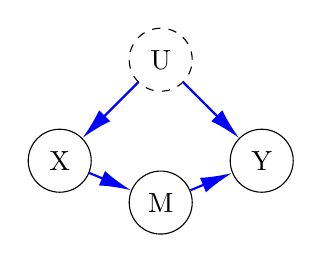
\begin{tikzpicture}[node distance=1cm]
                    \node[node, dashed] (u) {U};
                    \node[node, below left=of u] (x) {X};
                    \node[node, below=of u] (m) {M};
                    \node[node, below right=of u] (y) {Y};
                    
                    \draw[causal] (u) -- (x);
                    \draw[causal] (u) -- (y);
                    \draw[causal] (x) -- (m);
                    \draw[causal] (m) -- (y);
                \end{tikzpicture}
            \end{center}
        \end{column}
    \end{columns}
\end{frame}


\begin{frame}{Frontdoor Example: Smoking and Lung Cancer}
    \begin{columns}
        \begin{column}{0.6\textwidth}
            \begin{itemize}
                \item Does smoking cause lung cancer?
                \item Problem: Genetic factors may cause both smoking behavior and cancer susceptibility
                \item Solution: Use frontdoor criterion with tar deposits as mediator
            \end{itemize}
            
            \begin{exampleblock}{Logic}
                Smoking $\rightarrow$ Tar deposits in lungs $\rightarrow$ Lung cancer
            \end{exampleblock}
            
            % \begin{alertblock}{Key Insight}
            %     All causal effect of smoking on cancer goes through tar deposits - genes don't directly affect tar
            % \end{alertblock}
        \end{column}
        \begin{column}{0.4\textwidth}
            \begin{center}
                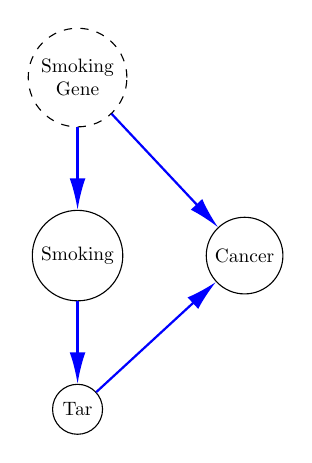
\begin{tikzpicture}[node distance=1.5cm, scale=0.7, transform shape]
                    \node[node] (smoking) {Smoking};
                    \node[node, dashed, above=of smoking, align=center] (gene) {Smoking\\Gene};
                    \node[node, below=of smoking] (tar) {Tar};
                    \node[node, right=of smoking] (cancer) {Cancer};
                    
                    \draw[causal] (gene) -- (smoking);
                    \draw[causal] (gene) -- (cancer);
                    \draw[causal] (smoking) -- (tar);
                    \draw[causal] (tar) -- (cancer);
                \end{tikzpicture}
            \end{center}
        \end{column}
    \end{columns}
\end{frame}

\begin{frame}{Frontdoor Example 2: Marketing and Sales}
    \begin{columns}
        \begin{column}{0.6\textwidth}
            \begin{itemize}
                \item Does advertising spending increase sales?
                \item Problem: Economic conditions affect both marketing budgets and consumer spending
                \item Solution: Use frontdoor criterion with brand awareness as mediator
            \end{itemize}
            
            \begin{exampleblock}{Logic}
                Advertising $\rightarrow$ Brand awareness $\rightarrow$ Product sales
            \end{exampleblock}
            
            % \begin{alertblock}{Key Insight}
            %     Economic conditions don't directly affect brand awareness - only through advertising spend
            % \end{alertblock}
        \end{column}
        \begin{column}{0.4\textwidth}
            \begin{center}
                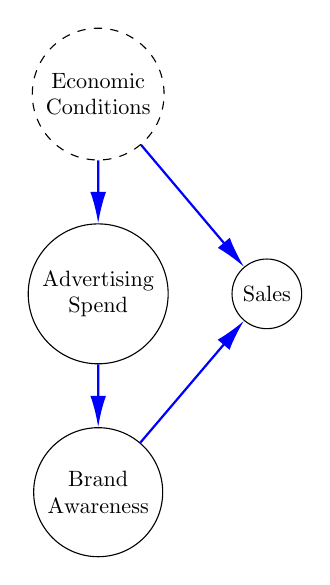
\begin{tikzpicture}[node distance=1cm, scale=0.8, transform shape]
                    \node[node, align=center] (advertising) {Advertising\\Spend};
                    \node[node, dashed, above=of advertising, align=center] (economy) {Economic\\Conditions};
                    \node[node, below=of advertising, align=center] (awareness) {Brand\\Awareness};
                    \node[node, right=of advertising] (sales) {Sales};
                    
                    \draw[causal] (economy) -- (advertising);
                    \draw[causal] (economy) -- (sales);
                    \draw[causal] (advertising) -- (awareness);
                    \draw[causal] (awareness) -- (sales);
                \end{tikzpicture}
            \end{center}
        \end{column}
    \end{columns}
\end{frame}


\begin{frame}{Instrumental Variables}
    \begin{columns}
        \begin{column}{0.6\textwidth}
            \begin{itemize}
                \item Used when there are \textbf{unobserved confounders}
                \item Z is an instrument if:
                \begin{enumerate}
                    \item Z affects X (relevance)
                    \item Z affects Y only through X (exclusion)
                    \item Z is unrelated to U (exogeneity)
                \end{enumerate}
            \end{itemize}
            
            
        \end{column}
        \begin{column}{0.4\textwidth}
            \begin{center}
                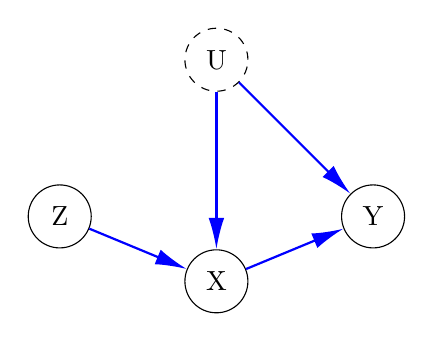
\begin{tikzpicture}[node distance=2cm]
                    \node[node, dashed] (u) {U};
                    \node[node, below left=of u] (z) {Z};
                    \node[node, below=of u] (x) {X};
                    \node[node, below right=of u] (y) {Y};
                    
                    \draw[causal] (u) -- (x);
                    \draw[causal] (u) -- (y);
                    \draw[causal] (z) -- (x);
                    \draw[causal] (x) -- (y);
                \end{tikzpicture}
            \end{center}
        \end{column}
    \end{columns}
\end{frame}

% Acemoglu et al. - Settler Mortality and Institutions
\begin{frame}{IV Example 1: Colonial Origins of Development}
    \begin{columns}
        \begin{column}{0.6\textwidth}
            \begin{itemize}
                \item \textbf{Acemoglu, Johnson, Robinson (2001)}
                \item How do institutions affect development?
                \item Problem: Good institutions and high GDP could both be caused by unobserved factors
                \item Solution: Instrument settler mortality
            \end{itemize}
            
            \begin{exampleblock}{Logic}
                High settler mortality → Extractive institutions → Poor modern institutions → Low GDP today
            \end{exampleblock}
        \end{column}
        \begin{column}{0.4\textwidth}
            \begin{center}
                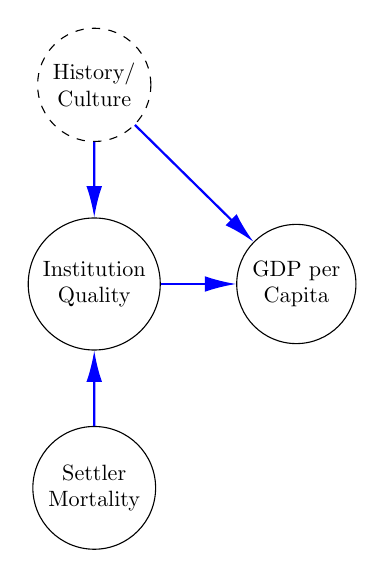
\begin{tikzpicture}[node distance=1.2cm, scale=0.8, transform shape]
                    \node[node, align=center] (x) {Institution\\Quality};
                    \node[node, dashed, above=of x, align=center] (u) {History/\\Culture};
                    \node[node, below=of x, align=center] (z) {Settler\\Mortality};
                    \node[node, right=of x, align=center] (y) {GDP per\\Capita};
                    
                    \draw[causal] (u) -- (x);
                    \draw[causal] (u) -- (y);
                    \draw[causal] (z) -- (x);
                    \draw[causal] (x) -- (y);
                \end{tikzpicture}
            \end{center}
        \end{column}
    \end{columns}
\end{frame}
% Angrist & Krueger - Quarter of Birth
\begin{frame}{IV Example 2: Returns to Education}
    \begin{columns}
        \begin{column}{0.6\textwidth}
            \begin{itemize}
                \item \textbf{Angrist \& Krueger (1991)}
                \item What is the causal effect of education on earnings?
                \item Problem: Ability affects both education and earnings
                \item Solution: Use quarter of birth as instrument
            \end{itemize}
            
            \vspace{0.3cm}
            
            \begin{exampleblock}{Logic}
                Born in Q4 → Start school older → Drop out with less education (due to compulsory schooling laws)
            \end{exampleblock}
        \end{column}
        \begin{column}{0.4\textwidth}
            \begin{center}
                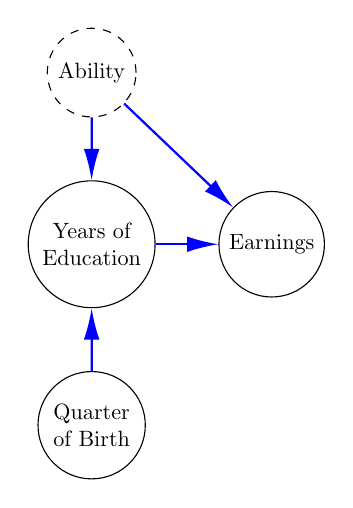
\begin{tikzpicture}[node distance=1cm, scale=0.8, transform shape]
                    \node[node, align=center] (x) {Years of\\Education};
                    \node[node, dashed, above=of x] (u) {Ability};
                    \node[node, below=of x, align=center] (z) {Quarter\\of Birth};
                    \node[node, right=of x] (y) {Earnings};
                    
                    \draw[causal] (u) -- (x);
                    \draw[causal] (u) -- (y);
                    \draw[causal] (z) -- (x);
                    \draw[causal] (x) -- (y);
                \end{tikzpicture}
            \end{center}
        \end{column}
    \end{columns}
\end{frame}

% Card - Distance to College
\begin{frame}{IV Example 3: College Proximity and Returns to Education}
    \begin{columns}
        \begin{column}{0.6\textwidth}
            \begin{itemize}
                \item \textbf{Card (1995)}
                \item Alternative approach to estimating returns to education
                \item Problem: Family background affects both education and earnings
                \item Solution: Use distance to nearest college as instrument
            \end{itemize}
            
            \vspace{0.3cm}
            
            \begin{exampleblock}{Logic}
                Living near a college → Lower cost of attendance → More likely to attend → Higher earnings
            \end{exampleblock}
        \end{column}
        \begin{column}{0.4\textwidth}
            \begin{center}
                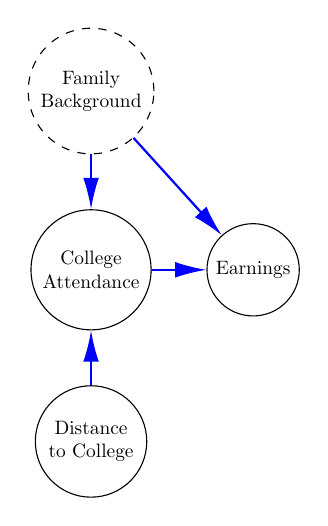
\begin{tikzpicture}[node distance=1cm, scale=0.7, transform shape]
                    \node[node, align=center] (x) {College\\Attendance};
                    \node[node, dashed, above=of x, align=center] (u) {Family\\Background};
                    \node[node, below=of x, align=center] (z) {Distance\\to College};
                    \node[node, right=of x] (y) {Earnings};
                    
                    \draw[causal] (u) -- (x);
                    \draw[causal] (u) -- (y);
                    \draw[causal] (z) -- (x);
                    \draw[causal] (x) -- (y);
                \end{tikzpicture}
            \end{center}
        \end{column}
    \end{columns}
\end{frame}

\begin{frame}{IV Example 4 Example: Job Training Partnership Act (JTPA)}
    \begin{columns}
    \begin{column}{0.6\textwidth}
        \begin{itemize}
            \item \textbf{JTPA Evaluation Study}
            \item How does job training affect earnings?
            \item Problem: Motivation is unobserved confounder
            \item Solution: Use frontdoor criterion with "showing up" as mediator
        \end{itemize}
        
        \begin{exampleblock}{Logic}
            Random assignment $\rightarrow$ Actually showing up $\rightarrow$ Job training received $\rightarrow$ Higher earnings
        \end{exampleblock}
        
    \end{column}
    \begin{column}{0.4\textwidth}
        \begin{center}
            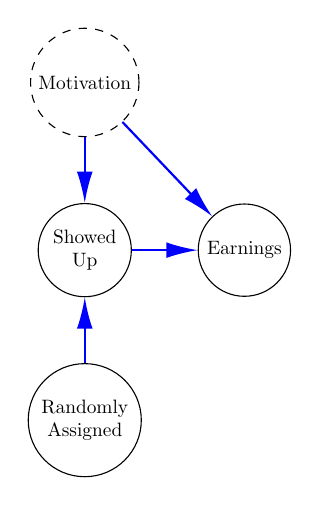
\begin{tikzpicture}[node distance=1.2cm, scale=0.7, transform shape]
                \node[node, align=center] (showed) {Showed\\Up};
                \node[node, below=of showed, align=center] (assigned) {Randomly\\Assigned};
                \node[node, dashed, above=of showed] (motivation) {Motivation};
                \node[node, right=of showed] (earnings) {Earnings};
                
                \draw[causal] (motivation) -- (showed);
                \draw[causal] (motivation) -- (earnings);
                \draw[causal] (assigned) -- (showed);
                \draw[causal] (showed) -- (earnings);
            \end{tikzpicture}
        \end{center}
    \end{column}
\end{columns}
\end{frame}

\begin{frame}{Summary}
    \begin{itemize}
        \item DAGs provide a visual language for causal reasoning
        \item Different structures (chains, forks, colliders) have different statistical properties
        \item Backdoor criterion helps identify valid control sets
        \item Frontdoor criterion and instrumental variables help when backdoor fails
        \item Understanding these concepts prevents common pitfalls in causal inference
    \end{itemize}
    
    \vspace{0.5cm}
    
    \begin{center}
        \Large{\textbf{Questions?}}
    \end{center}
\end{frame}

\end{document}